\section{GAUSFIT Gaussian Curve Fit}

\subsection{Usage}

The \verb|gausfit| routine has the following syntax
\begin{verbatim}
  [mu,sigma,dc,gain,yhat] = gausfit(t,y,w,mug,sigmag,dcg,gaing).
\end{verbatim}
where the required inputs are
\begin{itemize}
\item  \verb|t| - the values of the independant variable (e.g., time samples)

\item  \verb|y| - the values of the dependant variable (e.g., f(t))

\end{itemize}
The following inputs are all optional, and default values are
available for each of them.
\begin{itemize}
\item  \verb|w| - the weights to use in the fitting (set to ones if omitted)

\item  \verb|mug| - initial estimate of the mean

\item  \verb|sigmag| - initial estimate of the sigma (standard deviation)

\item  \verb|dcg| - initial estimate of the DC value

\item  \verb|gaing| - initial estimate of the gain

\end{itemize}
The fit is of the form \verb|yhat=gain*exp((t-mu).^2/(2*sigma^2))+dc|.
The outputs are 
\begin{itemize}
\item  \verb|mu| - the mean of the fit

\item  \verb|sigma| - the sigma of the fit

\item  \verb|dc| - the dc term of the fit

\item  \verb|gain| - the gain of the gaussian fit

\item  \verb|yhat| - the output samples (the Gaussian fits)

\end{itemize}
Because the fit is nonlinear, a good initial guess is critical to
convergence of the solution.  Thus, you can supply initial guesses
for each of the parameters using the \verb|mug|, \verb|sigmag|, \verb|dcg|, 
\verb|gaing| arguments.  Any arguments not supplied are estimated using 
a simple algorithm. In particular, the DC value is estimated by 
taking the minimum value  from the vector \verb|y|.  The gain is 
estimated from the range of \verb|y|.  The mean and standard deviation 
are estimated using the first and second order moments of \verb|y|.
This function uses \verb|fitfun|.
\subsection{Example}

Suppose we want to fit a cycle of a cosine using a Gaussian shape.
@>
Which results in the following plot


\centerline{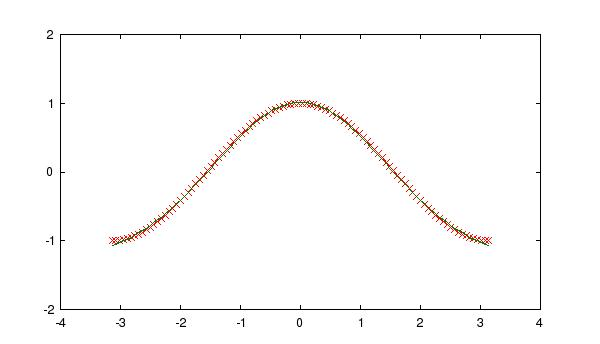
\includegraphics[width=8cm]{gausfit1}}

